\documentclass{article}

\usepackage{Sweave}
\begin{document}
\Sconcordance{concordance:Report.tex:Report.Rnw:%
1 2 1 1 0 73 1}



\title{Final Project}
\author{Joseph Francia, Priscilla Hartono, Nicholas Saber, Andrea Widjaja}
\maketitle

\section{Abstract}
This report is the third and final project of STAT 159, Reproducible and Collaborative Statistical Data Science, taught by Professor Gaston Sanchez in the fall of 2016 at UC Berkeley. STAT 159 focuses on the collaborative work and the ability to reproduce valuable data.

This paper consists of six parts: abstract, introduction, data, methods, analysis, results, conclusion. We used College Scorecard data, which was developed by the U.S. Department of Education (under Obama’s Administration) to provide “key indicators about the cost and value of institutions across the country to help students choose a school that is well-suited to meet their needs, priced affordably, and is consistent with their educational and career goals”. We used the data set corresponding to the 2014-2015 academic year because it is the most recent dataset we have access to. Meanwhile, in order to understand each variable, we referred to the data dictionary provided by College Scorecard. 


\section{Introduction}
Suppose we are Public Policy Researchers hired by the government. The government is interested in boosting graduation rates across the nation. However, its resources are limited, and the government is not sure how to spend its money. As a result, we are tasked with determining which variables affect a college’s graduation rate the most. In addition, the government wants to see how these variables might change if we were to look at graduation rates of people with different ethnicities. For instance, are the variables that affect Black people's graduation rates the same as the variables that affect Asian people's graduation rates? In order to answer these questions, the government wants us to build an interactive web application that allows a non-technical user to find the relevant variables for a specific ethnicity's graduation rates. 


\section{Data}

$College Scorecard$ has extensive data on colleges' admissions rates, graduation rates, and even the distribution of students based on race, income, and status from 1996 until 2015. For this project, we chose the most recent dataset, $MERGED2014_15_PP.csv$, which consists of 2014-2015 data. There are 7703 colleges in the dataset, and each college has 1743 attributes/variables of interest.

Before starting any analysis, we first cleaned the data by filtering out data we did not need. For instance, the government, our client, is only interested in analyzing graduation rates of students in public schools. As a result, we removed all private universities and colleges from our analysis. In addition, in order to use more consistent and reliable data, we futher filtered data choosing only main campuses, and colleges that award predominently bachelor degrees.

Because the data has so many variables, there are quite a few redundancies in the data. As a result, we removed quite a few variables from our dataset and only used the variables that we deemed relevant for our analysis. The predictors we selected were ACT and SAT scores, percentage of degrees awarded in each major, share of enrollment for each race, price of each college and number of students from each income group. We also created histograms for each of these quantitative variables.Below is a histogram of SAT scores for those who attended a public university:

\begin{figure}[!htb]
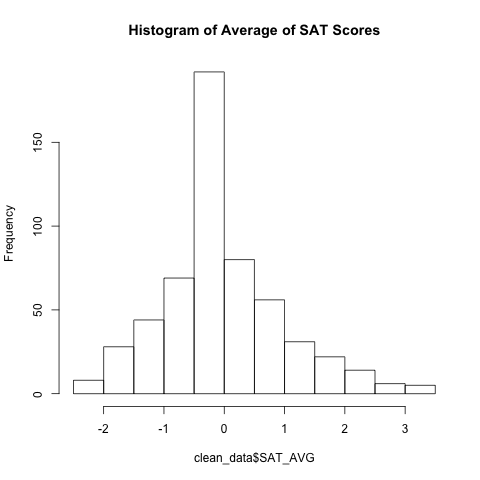
\includegraphics{../images/histogram_SAT_avg.png}
\end{figure}

Our response variable, meanwhile, is graduation rate rate and for further analysis we included the graduation rates specific to an ethnicity (Black, Asian, Hispanic, etc.). Below, I've show histograms for the graduation rates for each enthnicity:


\begin{figure}[!htb]
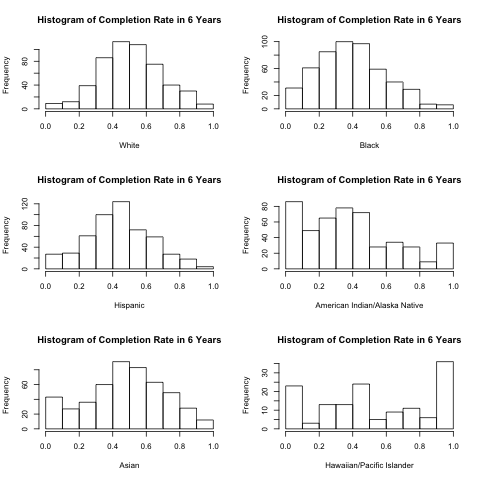
\includegraphics{../images/histogram_race_completion.png}
\end{figure}

While the above histograms are important, we're not merely interested in pointing out the differences in graduation rates between ethnicities. Rather, we're interested in finding the variables that motivate these differences. In the next section, I'll discuss the specific methods that we used for variable selection.


\section{Methodology}

So how exactly do we go about finding the variables that are relevant for graduation rates? It turns out that we can use a few different linear regression methods in order to accomplish this task.\\

\subsection{Lasso Regression}
Lasso Regression is essentially just a slight modification of Least-Squares Regression. In Least-Squares, the optimal solution is the beta vector that minimizes the sum of squared residuals. Because Lasso Regression's minimization problem is slightly different from least-squares, the optimal solution for Lasso is the beta vector that minimizes both the sum of squared residuals (bias) and the absolute norm of the beta vector (model complexity). In addition to possibly performing better from a prediction standpoint, the solution to Lasso has the added benefit of setting multiple beta coefficients equal to zero. The variables that correspond to these beta coefficients of zero are usually interpreted as having a minimal impact on the response variable.

\subsection{P-Values}
While p-values are usually associated with hypothesis testing, they can actually also be used for variable selection as well. For instance, imagine that we're in the linear regression setting where we have p explanatory variables, n observations, and one response variable y. In order to find the variable with the most explanatory power, lets run p regressions where we regress y individually on every single explanatory variable. We then compare these p regressions and select the variable with the beta coefficient that has the smallest p-value. Lets call this variable X1. In order to find the variable with the 2nd most explanatory power, we can run p-1 regressions where we regress y on X1 and a second explanatory variable. We then select the variable with the beta coefficient that has the smallest p-value. This variable can be interpreted as the second most important explanatory variable. We can iterate this process until we're satisfied with the number of relevant explanatory variables we have. While this forward stepwise selection algorithm is greedy and not necessarily optimal, it performs fairly decently and is more feasible than an exhaustive approach.

\subsection{BIC}
BIC (Bayesian Information Criterion) is a criterion for model selection. In a subset of models, the model with the lowest BIC value is deemed the best model. BIC is composed of both a bias term and a model complexity term. As a result, in order to achieve a low BIC, a model has to do a decent job of minimizing bias without too much model complexity. While BIC is normally used for model selection, it can also do a decent job at variable selection. Using the forward stepwise selection algorithm
described in the previous subsection, we would sequentially add a variable to the model, and this was the variable that decreased BIC the most. We would stop adding variables to the model once they started to increase the BIC of our model.

\section{Analysis}
So now that we've gone over each variable selection method, how do we know which one to use? We could see how each model (Lasso, P Value-based forward selection, BIC-based forward selection) performs from a predictive standpoint and use the model that has the most predictive power. However, the model that has the most predictive power is not necessarily the model that is the best at variable selection. The optimal model for variable selection is the model that is able to most accurately estimate beta coefficients for our explanatory variables. Unfortunately, given that we don't know each explanatory variable's true effect on graduation rate, there is no way for us to check how accurate our beta coefficient estimates are. As a result, there's no simple way for us to pick the model that is the best at variable selection.

All is not lost, however. While we may not be able to pick a single model to use for variable selection, we can just use all of 3 of our models. As a result, each model will identify a set of relevant explanatory variables. If a subset of these variables appear in all 3 of our models, we can identify these variables as extremely relevant to graduation rates. In the next section, we're going to go over how we used our Shiny R app to help us find the relevant variables for graduation rates.


\section{Results}
Once we figured out which variable selection methods we wanted to use and how we wanted to use them, we were then able to implement them using a Shiny R App. A screenshot of the Shiny R app at the end of the report shows exactly the options that a user has when running the web application.

\begin{figure}[!htb]
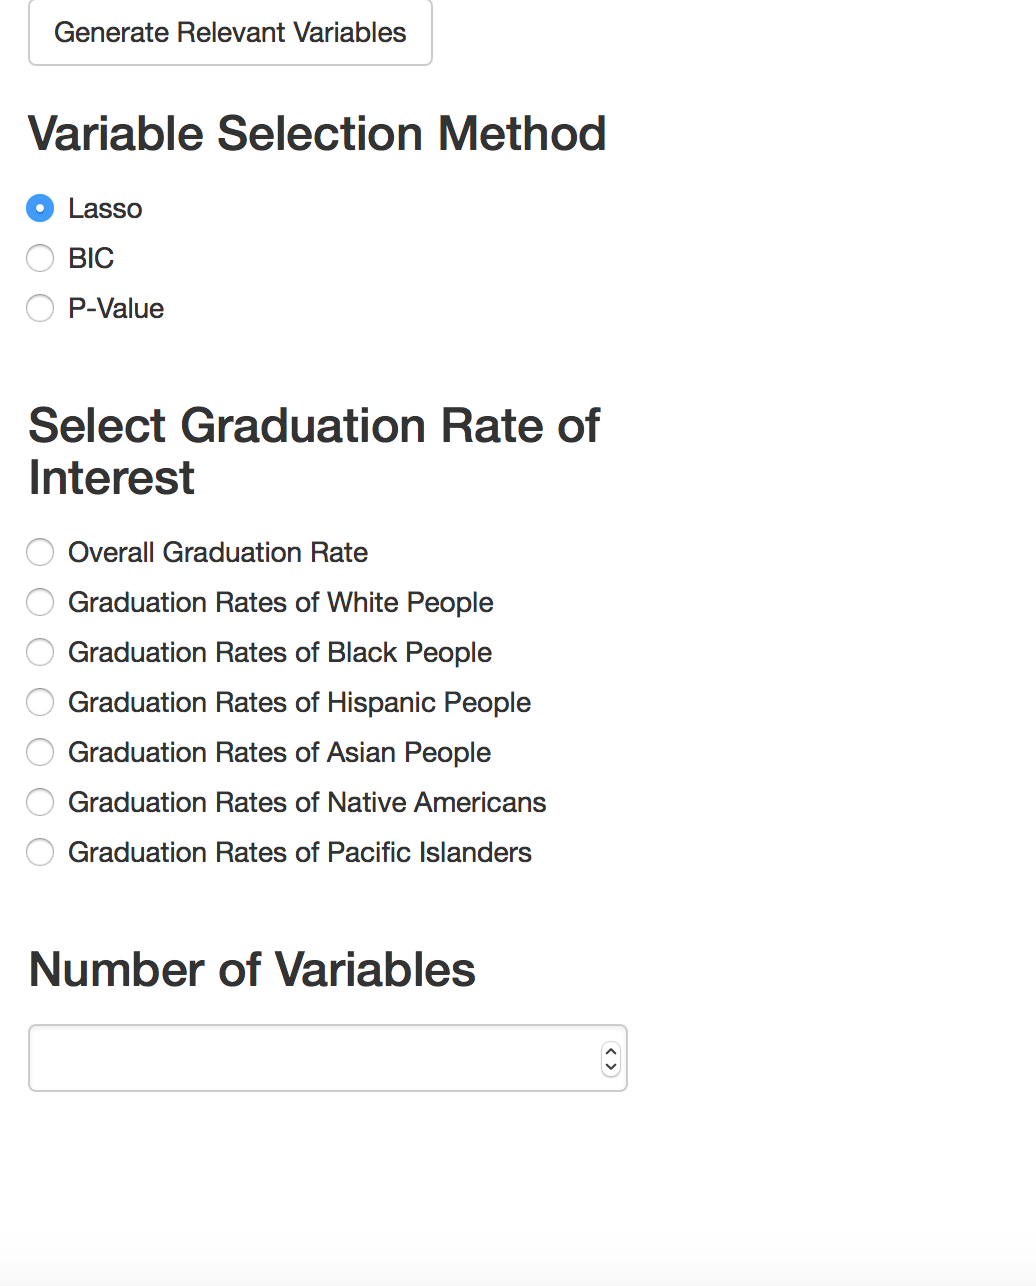
\includegraphics{../images/screenshot.png}
\end{figure}


The Shiny R App will then output the specified number of relevant variables for the specified graduation rate. For instance, lets say we were interested in finding the 5 most relevant explanatory variables for the overall graduation rate. Then, we could get 3 sets of 5 explanatory variables (one set for each variable selection method). It turns out that the only explanatory variable that appears in all 3 variable selection methods is the SAT average variable, which has a strong positive effect on graduation rates. This makes sense because intuitively, SAT scores have a strong correlation with high academic performance, which is essential to graduating. 

\section{Conclusion}
As consultants hired by the U.S. government, we didn't want to just provide a static analysis that would list out the variables relevant to graduation rates. Rather, we wanted to create a dynamic web application that would allow non-technical government officials to explore education data on their own. Users merely need to input the number of relevant variables they want to look at and the type of graduation rate that they are interested in analyzing. In addition to simplicity, the Shiny R Web app has the added benefit of providing reproducible analysis with different datasets. For instance, in the context of this project, the Shiny R App deals with data from the 2014-2015 academic year. However, if the U.S. government a few years from now were interested in the 2017-2018 academic year, the government could also use our web application to analyze the relevant variables for graduation rates in that academic year. The reproducibility of our Shiny R App is, in my opinion, its strongest suit, and will allow it to be relevant for our government clients for years to come.

\end{document}
